

\actTitle{Worksheet 2.1A}


\noindent \textbf{Instructions:}  Work together in groups of  3 or 4 to complete the following problems.




\begin{enumerate}
\item Given $f(x)=(x+2)^2-1$.
\begin{enumerate}
\item Determine whether the graph of the parabola opens upward or downward.\\[.3in]
\item Identify the vertex.\\[.3in]
\item Determine the $x$-intercept(s).\\[1in]
\item Determine the $y$-intercept.\\[.5in]
\item Sketch the function.\\
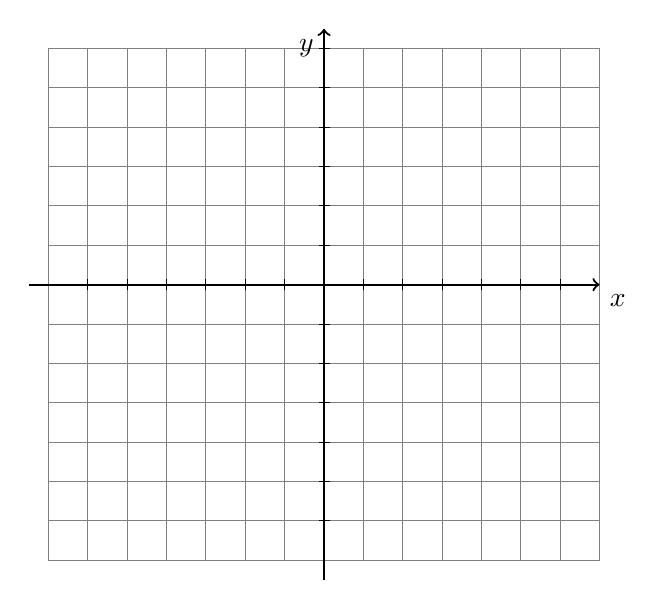
\begin{tikzpicture}[y=.5cm, x=0.5cm,font=\sffamily]
    %% ticks
    \draw[step = 1, gray] (-7,-7) grid (7,6);
    %% axis
    \draw[thick,->] (-7.5,0) -- coordinate (x axis mid) (7,0) node[anchor = north west] {$x$};
    \draw[thick,->] (0,-7.5) -- coordinate (y axis mid) (0,6.5) node[anchor = north east] {$y$};
    \foreach \y in {-6,-5,...,-1,1,2,...,6} {
      \draw (2pt, \y) -- (-2pt, \y);
    }
    \foreach \x in {-6,-5,...,-1,1,2,...,6} {
      \draw (\x,2pt) -- (\x,-2pt);
    }

\end{tikzpicture}

\item Determine the axis of symmetry.\\


\end{enumerate}


\newpage

\item Find the quadratic function with the given vertex and point.  Put your answer in standard (vertex) form.
\begin{enumerate}
\item Vertex $(0,0)$ passing through $(-2,8)$.

\vfill


\item  Vertex $(2,0)$ passing through $(1,3)$.
\vfill
 
 \item Vertex $(2,5)$ passing through $(3,7)$.
 \vfill
 
 \item  Vertex $(-3,4)$ passing through $(0,0)$.
 
 \vfill
 \end{enumerate}

\newpage

\item In each problem below, complete the square and then use that work to find the vertex of the graph of the quadratic function.
\begin{enumerate}
\item $y=x^2+4x$\vfill
\item $y=x^2-2x+2$\vfill
\item $y=6x-10-x^2$\vfill
\item  $y=-2x^2+16x-29$ \vfill

\end{enumerate}




\vfill

\newpage 

\item Find the equation for the parabolas below.  Put your answers in standard form.
\begin{enumerate}
\item $y=$\\



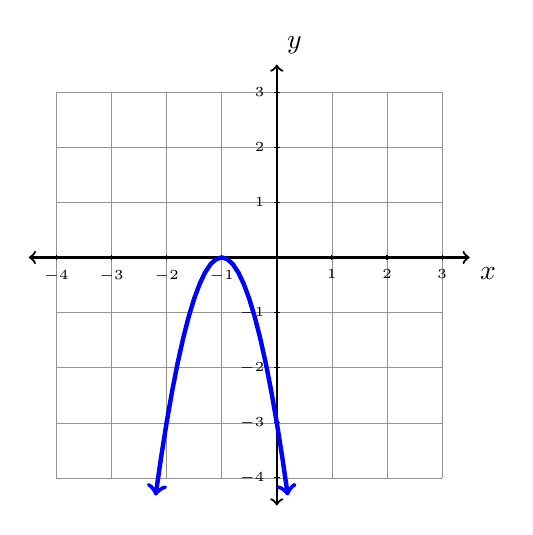
\begin{tikzpicture}[y=.7cm, x=.7cm,font=\sffamily,
	mydot/.style={
    circle,
    fill=white,
    draw,
    outer sep=0pt,
    inner sep=1.5pt
  }]
    %% Add a grid
    \draw[step = 1, gray, very thin,opacity=0.85] (-4, -4) grid (3, 3);
 	%% Draw the axes
	\draw[thick,<->] (-4.5,0) -- coordinate (x axis mid) (3.5,0) node[anchor = north west] {$x$};
    \draw[thick,<->] (0,-4.5) -- coordinate (y axis mid) (0,3.5) node[anchor = south west] {$y$};
    %% Label the y axis
    \foreach \y in {-4,...,-1,1,2,...,3} {
      \draw (1pt, \y) -- (-1pt, \y) node[anchor =  east] {\tiny$\y$};
    }
    %% Label the x axis
    \foreach \x in {-4,...,-1,1,2,...,3} {
      \draw (\x,1pt) -- (\x,-1pt) node[anchor = north] {\tiny$\x$};
    }
    %% Draw the function.
   \begin{scope}
  %       \draw[very thick,black] (-3,2) -- (1,1);
 %        \draw[very thick,black] (3.05,1.05) -- (4,3);
    %semi-circle
  %       \draw[very thick, black] (1,1) arc [radius=1, start angle=180, end angle= 5];
     %function
         \draw[ultra thick, blue, <->, domain=-2.2:.2] plot (\x, {-3*(\x+1)^2});
      
     %dots
%       \fill[blue] (2, 4) circle[radius=0.5ex];
     %  \fill[black] (1,1) circle[radius=0.5ex];
     %    \fill[black] (4,3) circle[radius=0.5ex];
     %     \draw[very thick, black] (3,1) circle[radius=0.5ex];


    \end{scope}

    %%\node[above=0.1cm] at (-2,2 )   {\nextXValue};

  \end{tikzpicture}



\item $y=$\vspace{1em}


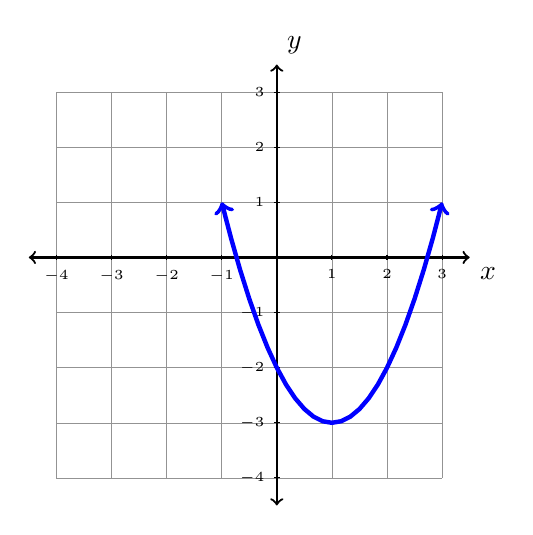
\begin{tikzpicture}[y=.7cm, x=.7cm,font=\sffamily,
	mydot/.style={
    circle,
    fill=white,
    draw,
    outer sep=0pt,
    inner sep=1.5pt
  }]
    %% Add a grid
    \draw[step = 1, gray, very thin,opacity=0.85] (-4, -4) grid (3, 3);
 	%% Draw the axes
	\draw[thick,<->] (-4.5,0) -- coordinate (x axis mid) (3.5,0) node[anchor = north west] {$x$};
    \draw[thick,<->] (0,-4.5) -- coordinate (y axis mid) (0,3.5) node[anchor = south west] {$y$};
    %% Label the y axis
    \foreach \y in {-4,...,-1,1,2,...,3} {
      \draw (1pt, \y) -- (-1pt, \y) node[anchor =  east] {\tiny$\y$};
    }
    %% Label the x axis
    \foreach \x in {-4,...,-1,1,2,...,3} {
      \draw (\x,1pt) -- (\x,-1pt) node[anchor = north] {\tiny$\x$};
    }
    %% Draw the function.
   \begin{scope}
  %       \draw[very thick,black] (-3,2) -- (1,1);
 %        \draw[very thick,black] (3.05,1.05) -- (4,3);
    %semi-circle
  %       \draw[very thick, black] (1,1) arc [radius=1, start angle=180, end angle= 5];
     %function
         \draw[ultra thick, blue, <->, domain=-1:3] plot (\x, {(\x-1)^2-3});
      
     %dots
%       \fill[blue] (2, 4) circle[radius=0.5ex];
     %  \fill[black] (1,1) circle[radius=0.5ex];
     %    \fill[black] (4,3) circle[radius=0.5ex];
     %     \draw[very thick, black] (3,1) circle[radius=0.5ex];


    \end{scope}

    %%\node[above=0.1cm] at (-2,2 )   {\nextXValue};

  \end{tikzpicture}


%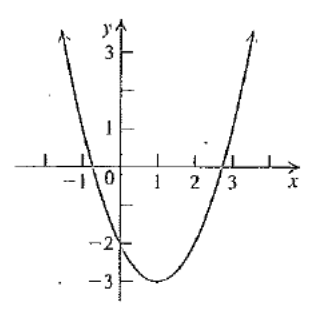
\includegraphics{parabola-b}

\item $y=$\\


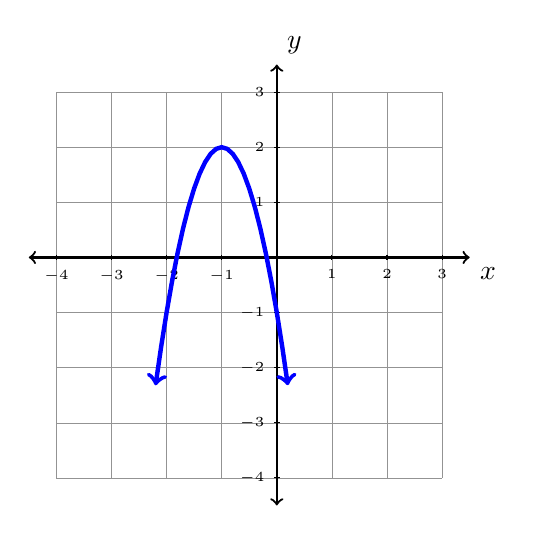
\begin{tikzpicture}[y=.7cm, x=.7cm,font=\sffamily,
	mydot/.style={
    circle,
    fill=white,
    draw,
    outer sep=0pt,
    inner sep=1.5pt
  }]
    %% Add a grid
    \draw[step = 1, gray, very thin,opacity=0.85] (-4, -4) grid (3, 3);
 	%% Draw the axes
	\draw[thick,<->] (-4.5,0) -- coordinate (x axis mid) (3.5,0) node[anchor = north west] {$x$};
    \draw[thick,<->] (0,-4.5) -- coordinate (y axis mid) (0,3.5) node[anchor = south west] {$y$};
    %% Label the y axis
    \foreach \y in {-4,...,-1,1,2,...,3} {
      \draw (1pt, \y) -- (-1pt, \y) node[anchor =  east] {\tiny$\y$};
    }
    %% Label the x axis
    \foreach \x in {-4,...,-1,1,2,...,3} {
      \draw (\x,1pt) -- (\x,-1pt) node[anchor = north] {\tiny$\x$};
    }
    %% Draw the function.
   \begin{scope}
  %       \draw[very thick,black] (-3,2) -- (1,1);
 %        \draw[very thick,black] (3.05,1.05) -- (4,3);
    %semi-circle
  %       \draw[very thick, black] (1,1) arc [radius=1, start angle=180, end angle= 5];
     %function
         \draw[ultra thick, blue, <->, domain=-2.2:.2] plot (\x, {-3*(\x+1)^2+2});
      
     %dots
%       \fill[blue] (2, 4) circle[radius=0.5ex];
     %  \fill[black] (1,1) circle[radius=0.5ex];
     %    \fill[black] (4,3) circle[radius=0.5ex];
     %     \draw[very thick, black] (3,1) circle[radius=0.5ex];


    \end{scope}

    %%\node[above=0.1cm] at (-2,2 )   {\nextXValue};

  \end{tikzpicture}


%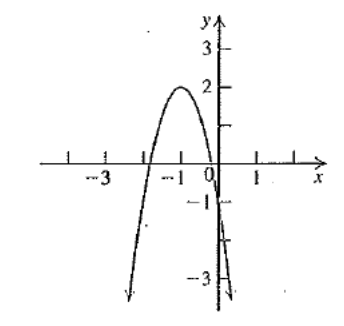
\includegraphics{parabola-c}
\end{enumerate}

\vfill

\newpage

\item Solve the following equations.
\begin{enumerate}
\item $x^2-10x+8=0$
\vfill 
\item $3x^2+6x=4$
\vfill
\item $x-3=\sqrt{1+2x^2}$
\vfill
\end{enumerate}

\end{enumerate}



